In questa sezione applicheremo il metodo dei minimi quadrati per ottenere un fit dei dati.
Il nostro scopo è ottenere una retta

\begin{equation}
	\mathcal{T}(m) \,=\, A + B m 
\end{equation}
%
dove $A$ è l'intercetta, mentre $B$ rappresenta il coefficiente angolare della retta. Se il coefficiente angolare $B$ della 
retta di fit risulterà compatibile con 0, sarà l'indicazione che la massa non influenza il periodo. 

\begin{SCfigure}
    \centering
    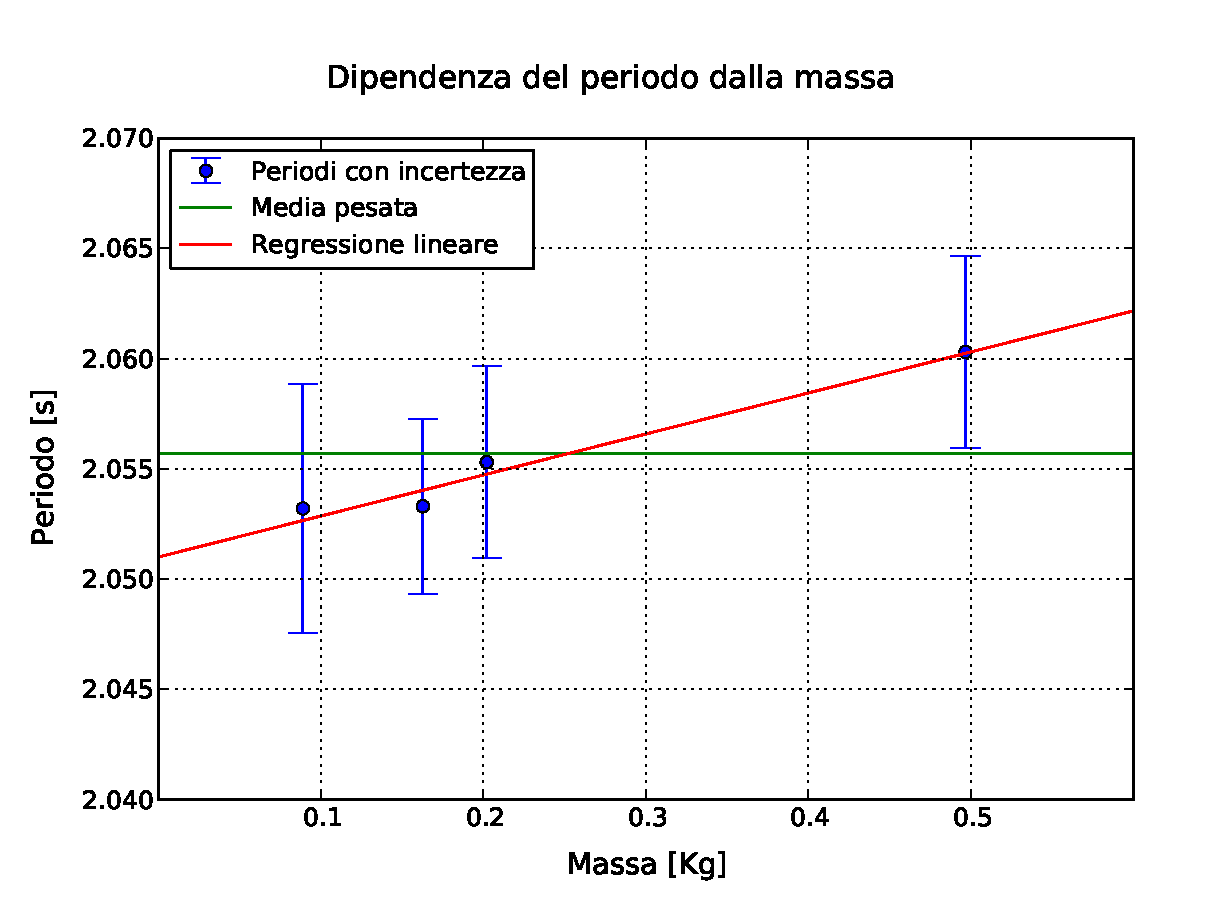
\includegraphics[width=110mm]{immagini/masse.pdf}
    \caption{Il seguente grafico rappresenta sull'asse delle ordinate le medie dei periodi relativi ad ogni
        singola massa, mentre sull'asse delle ascisse sono riportate le masse utilizzate. L'incertezza sul periodo
        è differente da misura a misure, mentre quella reativa alla massa è uguale per tutte, ed in particolare è
        l'incertezza tipo. La retta orizzontale verde rappresenta il valore (costante) della media pesata delle medie
        dei periodi $\mathcal{T}_w$, mentre in rosso è rappresentata la retta derivante dalla regressione lineare,
        ovvero la funzione $\mathcal{T}(m) = A + B\,m$.}
    \label{fig:masse_periodi}
\end{SCfigure}

%Finora abbiamo assunta veritiera l'ipotesi che il periodo di oscillazione del pendolo non dipende linearmente dalla massa applicata. Ciononostante ora vogliamo controllare se effettivamente sia così e quindi abbiamo deciso di fare una regressione lineare sulla funzine $f$ in modo da dare una stima ai parametri A e B e verificare che A risulti compatibile con il periodo del pendolo $\mathcal{T}$ trovato grazie alla media pesata e che il valore di B sia compatibie con lo 0 teorico.\\

Procediamo operativamente in questo modo per eseguire la regressione lieare:

\begin{itemize}
	\item{Grazie al grafico in figura \ref{fig:masse_periodi}, diamo una stima preliminare del parametro B, al fine di trasferire
        l'incertezza dalle masse ai periodi. Per avere una stima del parametro B calcoliamo il coefficiente angolare della retta che
        passa per il primo e ultimo punto, ovvero:
			\begin{equation*}
				B' \,=\, \frac{\mathcal{T}_4 - \mathcal{T}_1}{m_4 - m_1} \,\simeq\, \SI{0.02}{\second\per\kilo\gram}
			\end{equation*}
			%
			}
	\item{La funzione da minimizzare che misura la discrepanza è:
			\begin{equation}
                \sum_{i=1}^{\mathcal{N}} \frac{(\mathcal{T}_i - A - B m_i)}{(\delta \mathcal{T}_i^\text{tot})^2}	
                \label{eq:m_min_quad}
			\end{equation}
			%
            dove $\delta \mathcal{T}_i^\text{tot}$ viene ottenuta componendo
            l'incertezza $\delta \mathcal{T}_i$ e l'errore trasferito dal peso $B'\delta m$. Tuttavia, l'incertezza
            trasferita è trascurabile rispetto all'incertezza sul periodo poichè $\delta \mathcal{T}_i$ è dell'ordine di
            grandezza di $10^{-3}$ s mentre l'incertezza trasferita dalla massa è dell'ordine di $10^{-6}$ s.
            Quindi si ha che $\delta \mathcal{T}_i^\text{tot} = \delta \mathcal{T}_i$;}
	\item{Per quanto studiato in classe si ha che la il minimo di (\ref{eq:m_min_quad}) si ottiene per:

			\begin{equation*}
				A \,=\, \frac{(\sum_i w_i m_i^2)(\sum_i w_i \mathcal{T}_i) - (\sum_i w_i m_i)(\sum_i w_i m_i \mathcal{T}_i)}{\Delta}
                \,=\, \SI{2.051}{\second}
			\end{equation*}
			%
			\begin{equation*}
				B \,=\, \frac{(\sum_i w_i)(\sum_i w_i m_i \mathcal{T}_i) - (\sum_i w_i \mathcal{T}_i)(\sum_i w_i m_i)}{\Delta}
                \,=\, \SI{0.02}{\second\per\kilo\gram}
			\end{equation*}
			%
			dove:
			\begin{equation*}
				\Delta \,=\, (\sum_i w_i)(\sum_i w_i m_i^2) - (\sum_i w_i m_i)^2 \qquad \text{e} \qquad
				w_i \,=\, \frac{1}{(\delta \mathcal{T}_i)^2}
			\end{equation*}}
	\item{Inoltre abbiamo che le incertezze su A e B sono:

			\begin{equation*}
				\delta A \,=\, \sqrt{\frac{\sum_i w_i m_i^2}{\Delta}} = \SI{0.004}{\second}  \,\,\,\,\, e \,\,\,\,\,
				\delta B \,=\, \sqrt{\frac{\sum_i w_i}{\Delta}} = \SI{0.01}{\second\per\kilo\gram}
			\end{equation*}}
	\end{itemize} 
	Quindi possiamo riassumere i risultati di questa procedura in questo modo:

	\begin{equation*}
		A \,\pm\, \delta A \,=\, (2.051 \,\, \pm \,\, 0.004) \: \si{\second} \,\,\,\,\, e \,\,\,\,\,
		B \,\pm\, \delta B \,=\, (0.02 \,\, \pm \,\, 0.01) \: \si{\second\per\kilo\gram}
	\end{equation*}
	%
    Osserviamo che il valore stimato $B'$ è compatibile con il valore ricavato dalla regressione, perché i due valori
    sono uguali entro l'incertezza. Non è quindi necessario reiterare la procedura di fit.
    Il grafico in figura \ref{fig:masse_periodi} mostra la retta ottenuta dal fit.

\subsubsection{Test del chi quadro per la regressione}

Prima di verificare se il valore di $B$ ottenuto è compatibile con 0 e se risulta verificato che il periodo non dipende dalla massa,
eseguiamo il test del chi quadro sulla regressione appena calcolata per verificare se le incertezze sono state stimate correttamente.\\
%
Come già fatto nella sezione \ref{m_chi_pesata}, prendiamo un intervallo di confidenza del 95 \%, per cui la probabilità di falso allarme
è del 5 \%. In questo caso abbiamo 2 gradi di libertà, perché dai dati sono stati calcolati 2 parametri ($A$ e $B$). Calcolando l'intervallo
di accettazione a partire dal livello di confidenza si ottiene che il risultato del test è positivo il $\chi^2$ è compreso tra 0 a 5.99. \\
%
Il valore calcolato dai dati del chi quadro è:

\begin{equation*}
	\chi_{oss}^2 \,=\, \frac{\sum_{i=0}^{\mathcal{N}} (\mathcal{T}_i - A - Bm_i)^2}{(\delta \mathcal{T}_i)^2} \,=\, 0.06
\end{equation*}
%
Il chi quadro è molto basso, ma rientra nell'intervallo di valori ammissibili. Le incertezze sono quindi corrette.

\subsubsection{Compatibilità della regressione}

%Quindi non ci rimane altro che verificare se i due parametri così trovati risultano compatibili con quelli ipotizzati, ovvero A deve risultare compatibile con il periodo medio del pendolo calcolato grazie alla media pesata, mentre B deve risultare compatibile con lo 0 teorico. 

Verifichiamo ora che il coefficiente angolare B sia compatibile con lo 0 teorico.
Pertanto posto a priori un fattore di copertura $k = 3$:

\begin{itemize}
	%\item{calcoliamo la discrepanza $R$ tra $\mathcal{T}$ ed A, ottenendo:
	%		\begin{equation*}
	%			R \,=\, \mathcal{T} - A \,=\, 0.005 \,s
	%		\end{equation*}
			%
	%		}
	%\item{verificiamo ora se $R \leq k\,\sigma[R]$, dove:
	%		\begin{equation*}
	%			\sigma[R] \,=\, \sqrt{(\delta \mathcal{T})^2 + (\delta A)} \,=\, 0.004  \, s \bigotimes
	%		\end{equation*}
			%
	%		pertanto otteniamo che:
	%		\begin{equation*}
	%			R \leq k\,\sigma[R] \quad \text{in quanto} \quad 0.005 \, s \leq 0.013 \, s \bigotimes
	%		\end{equation*}
%WARNING! qualcosa non quadra nelle moltiplicazioni, sono giuste?			
			
			%
	%		e quindi $\mathcal{T}$ risulta compatibile con A}
	\item{troviamo ora la discrepanza $R$ tra $B$ ed il valore teorico 0, ottenendo:
			\begin{equation*}
				R \,=\, B - 0 \,=\, B \,=\, \SI{0.02}{\second\per\kilo\gram}
			\end{equation*}
			%
			}
	\item{controlliamo ora se $R \leq k\,\sigma[R]$, dove:
			\begin{equation*}
				\sigma[R] \,=\, \delta B \,=\, \SI{0.01}{\second\per\kilo\gram}	
			\end{equation*}
			%
			otteniamo che:
			\begin{equation*}
				R \leq k\,\sigma[R] \quad \text{in quanto} \quad 0.02 \leq 0.03
			\end{equation*}
			%
			e quindi $B$ risulta compatibile con lo 0 teorico}			
\end{itemize}
Grazie a questa breve analisi abbiamo verificato per la seconda volta (la prima è stata fatta con il test del chi quadro nel caso della media
pesata) che il periodo del pendolo non dipende dalla massa applicata.

%A =  2.0510
%B =  0.018602
%sigma_A =  0.0042932
%sigma_B =  0.014691
%chi2_fit =  0.057346
